\section{Несжимаемая жидкость}
\label{sec:p10}

В очень многих случаях течения жидкостей (и газов) их плотность можно считать
неизменяющейся, т. е. постоянной вдоль всего объема жидкости в течение всего
времени движения. Другими словами, в этих случаях при движении не происходит
заметных сжатий или расширений жидкости. О таком движении говорят как о движении
\textit{несжимаемой жидкости}.

Общие уравнения гидродинамики сильно упрощаются при применении их к несжимаемой
жидкости. Правда, уравнение Эйлера не меняет своего вида, если положить в нем
$\rho = \const$, за исключением только того, что в уравнении (\ref{eq:2.4}) можно внести
$\rho$ под знак градиента:
\begin{equation}
   \label{eq:10.1}
   \pd{\vv}{t} + \vnv = - \nabla \frac{p}{\rho} + \vect g
\end{equation}
Зато уравнение непрерывности принимает при $\rho = \const$ простой вид
\begin{equation}
   \label{eq:10.2}
   \Div \vv = 0.
\end{equation}

Поскольку плотность не является теперь неизвестной функцией, как это имеет
место в общем случае, то в качестве основной системы уравнений гидродинамики
несжимаемой жидкости можно выбрать уравнения, содержащие только скорость.
Такими уравнениями являются уравнение непрерывности (\ref{eq:10.2}) и уравнение (\ref{eq:2.11}):
\begin{equation}
   \label{eq:10.3}
   \pdt \rot \vv = \rot \vrv.
\end{equation}

Уравнение Бернулли тоже может быть написано для несжимаемой жидкости в более
простом виде. Уравнение (\ref{eq:10.1}) отличается от общего уравнения Эйлера (\ref{eq:2.9}) тем,
что вместо $\nabla w$ в нем стоит $\nabla(p/\rho)$. Поэтому мы можем сразу
написать уравнение Бернулли, заменив просто в (\ref{eq:5.4}) тепловую функцию
отношением $p/\rho$:
\begin{equation}
   \label{eq:10.4}
   \frac{v^2}{2} + \frac{p}{\rho} + gz = \const.
\end{equation}
Для несжимаемой жидкости можно писать $p/\rho$ вместо $w$ также и в выражении
(\ref{eq:6.3}) для потока энергии, которое принимает тогда вид
\begin{equation}
   \label{eq:10.5}
   \rho \vv \left( \frac{p}{\rho} + \frac{v^2}{2} \right).
\end{equation}
Действительно, согласно известному термодинамическому соотношению имеем для
изменения внутренней энргии выражение $d\varepsilon = T\; ds - p\;dV$; при $s =
\const$ и $V=1/\rho = \const$ имеем $d\varepsilon=0$, т. е.
$\varepsilon=\const$. Поскольку же постоянные члены в энергии несущественны, то
можно опустить $\varepsilon$ и в $w=\varepsilon+p/\rho$.

В особенности упрощаются уравнения для потенциального течения несжимаемой
жидкости. Уравнение (\ref{eq:10.3}) удовлетворяется при $\rot \vv = 0$ тождественно.
Уравнение же (\ref{eq:10.2}) при подстановке $\vv = \grad \varphi$ превращается в
\begin{equation}
   \label{eq:10.6}
   \Delta \varphi = 0,
\end{equation}
т. е. в уравнение Лапласа для потенциала $\varphi$ \footnote{Потенциал скорости был
впервые введен \em{Эйлером}. Им же было получено для этой величины уравнение вида
\ref{eq:10.6}, получившее впоследствии название уравнения Лапласа.}. К этому уравнению должны
быть добавлены граничные условия на поверхностях соприкосновения жидкости с
твердыми телами: на неподвижных твердых поверхностях нормальная к поверхности
компонента $v_n$ скорости жидкости должна быть равна нулю, а в общем случае
движущихся твердых тел $v_n$ должна быть равна проекции скорости движения тела
на направление той же нормали (эта скорость является заданной функцией времени).
Скорость $v_n$ равна, с другой стороны, производной от потенциала $\varphi$ по
направлению нормали: $v_n = \pd{\varphi}{n}$. Таким образом, граничные условия
гласят в общем случае, что $\pd{\varphi}{n}$ является на границах заданной
функцией времени и координат.

При потенциальном движении скорость связана с давлением уравнением (\ref{eq:9.3}).
В случае несжимаемой жидкости в этом уравнении можно писать $p/\rho$ вместо $w$:
\begin{equation}
   \label{eq:10.7}
   \pd{\varphi}{t} + \frac{v^2}{2} + \frac{p}{\rho} = f(t).
\end{equation}

\begin{wrapfigure}{l}{6cm}
% "l" or "r" for the side on the page.
% And the width parameter for the width of the image space.
  \centering
  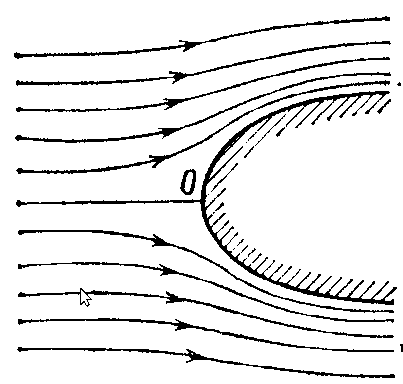
\includegraphics[width=6cm]{fig2}
  \caption{\label{fig:f2}}
\end{wrapfigure}

Отметим здесь следующее важное свойство потенциального движения несжимаемой
жидкости. Пусть через жидкость движется какое-нибудь твердое тело. Если
возникающее при этом течение жидкости является потенциальным, то это течение
зависит в каждый момент только от скорости движущегося тела в этот же момент
времени, но, например, не от его ускорения. Действительно, самое уравнение
(\ref{eq:10.6}) не содержит времени явно; время входит в решение лишь через граничные
условия, содержащие только скорость движущегося в жидкости тела.

Из уравнения Бернулли $v^2+p/\rho = \const$ видно, что при стационарном движении
несжимаемой жидкости (без поля тяжести) наибольшее значение давлений достигается
в точках, где скорость обращается в нуль. Такая точка обычно имеется на
поверхности обтекаемого жидкостью тела (точка $O$ на рис. 2) и называется
\textit{критической точкой}. Если $u$ - скорость натекающего на тело потока
жидкости (т. е. скорость жидкости на бесконечности), а $p_0$ - давление на
бесконечности, то давление в критической точке равно
\begin{equation}
   \label{eq:10.8}
   p_{max} = p_0 + \frac{\rho u^2}{2}.
\end{equation}

Если распределение скоростей в движущейся жидкости зависит только от двух
кородинат, скажем от $x$ и $y$, причем скорость параллельна везде плоскости
$xy$, то о таком течении говорят как о двухмерном или плоском. Для решения задач
о двухмерном течении несжимаемой жидкости иногда бывает удобным выражать
скорость через так называемую функцию тока. Из уравнения непрерывности
\[
   \Div \vv \equiv \pd{v_x}{x} + \pd{v_y}{y} = 0
\]
видно, что компоненты скорости могут быть написаны в виде производных
\begin{equation}
   \label{eq:10.9}
   v_x = \pd{\psi}{y},\; v_y = -\pd{\psi}{x}
\end{equation}
от некоторой функции $\psi(x,y)$, называемой \textit{функцией тока}. Уравнение
непрерывности при этом удовлетворяется автоматически. Уравнение же, которому
должна удовлетворять функция тока, получается подстановкой (\ref{eq:10.9}) в уравнение (\ref{eq:10.3})
\begin{equation}
   \label{eq:10.10}
   \pdt \nabla \psi -
   \pd{\psi}{x}\pd{\nabla\psi}{y}+
   \pd{\psi}{y}\pd{\nabla\psi}{x} = 0
\end{equation}

Зная функцию тока, можно непосредственно определить форму линий тока для
стационарного движения жидкости. Действительно, дифференциальное уравнение линий
тока (при двухмерном течении) есть
\[
   \frac{dx}{v_x} = \frac{dy}{v_y}
\]
или $v_y dx - v_x dy = 0$; оно выражает собой тот факт, что направление
касательной к линии тока в каждой точке совпадает с направлением скорости.
Подставляя сюда (\ref{eq:10.9}), получаем:
\[
   \pd{\psi}{x}dx + \pd{\psi}{y}dy = d\psi = 0,
\]
откуда $\psi = \const$. Таким образом, линии тока представляют собой семейство
кривых, получающихся приравниванием функции тока $\psi(x,y)$ произвольной
постоянной.

Если между двумя точками 1 и 2 в плоскости $x,y$ провести кривую, то поток
жидкости $Q$ через эту кривую определится разностью значений функции тока в этих
точках независимо от формы кривой. Действительно, если $v_n$ - проекция скорости
на нормаль к кривой в данной ее точке, то
\[
   Q = \rho \int_{1}^{2} v_n\;dl =
   \rho \int_{1}^{2} (-v_y\;dx + v_x\;dy) =
   \rho \int_{1}^{2} d\psi,
\]
или
\begin{equation}
   \label{eq:10.11}
   Q = \rho (\psi_2 - \psi_1).
\end{equation}
Мощные методы решения задач о плоском потенциальном обтекании несжимаемой
жидкостью различных профилей связаны с применением к ним теории функций
комплексного переменного\footnote{Подробное изложение этих методов и их многочисленных
применений может быть найдено во многих курсах и монографиях по гидродинамике с более
математическим уклоном. Здесь мы ограничимся лишь объяснением основной идеи метода}.
Основание для этих применений заключается в следующем.
Потенциал и функция тока связаны с компонентами скорости посредством
\footnote{Напомним, однако, что существование самой по себе функции тока связано
только с двумерностью течения, и отнюдь не требует его потенциальности.}
\[
   v_x=\pd{\varphi}{x}=\pd{\psi}{y},\; v_y = \pd{\varphi}{y}=-\pd{\psi}{x}.
\]
Но такие соотношения между производными функций $\varphi$ и $\psi$ с
математической точки зрения совпадают с известными условиями Коши-Римана,
выражающими собой тот факт, что комплексное выражение
\begin{equation}
   \label{eq:10.12}
   w = \varphi + i\psi
\end{equation}
является аналитической функцией комплексного аргумента $z=x+iy$. Это значит,
что функция $w(x)$ будет иметь в каждой точке определенную производную
\begin{equation}
   \label{eq:10.13}
   \D{w}{z} = \pd{\varphi}{x}+i \pd{\psi}{x} = v_x - iv_y.
\end{equation}

Функцию $w$ называют \textit{комплексным потенциалом}, а $\D{w}{z}$ -
комплексной скоростью. Модуль и аргумент последней определяют абсолютную
величину скорости $v$ и угол $\theta$ ее наклона к направлению оси $x$:
\begin{equation}
   \label{eq:10.14}
   \D{w}{z} = v e^{-i\theta}.
\end{equation}

На твердой поверхности обтекаемого контура скорость должна быть направлена по
касательной к нему. Другими словами, контур должен совпадать с одной из линий
тока, т. е. на нем должно быть $\psi = \const$; эту постоянную можно выбрать
равной нулю, и тогда задача об обтекании жидкостью заданного контура сводится к
определению аналитической функции $w(z)$, принимающей на этом контуре
вещественные значения. Более сложна постановка задачи в случаях, когда жидкость
имеет свободную поверхность (такой пример - см. задачу 9 к этому параграфу).

Интеграл от аналитической функции по какому-либо замкнутому контуру $C$ равен,
как известно, умноженной на $2\pi i$ сумме вычетов этой функции относительно ее
простых полюсов, расположенных внутри $C$; поэтому
\[
   \oint w'\;dz = 2\pi i \sum_{k} A_k,
\]
где $A_k$ - вычеты комплексной скорости. С другой стороны, имеем:
\begin{eqnarray}
   \oint w'\;dz =
   \oint (v_x - i v_y)(dx + i dy) = \\
   \oint (v_x dx + v_y dy) + i \oint (v_x dy - v_y dx).
\end{eqnarray}
Вещественная часть этого выражения есть не что иное, как циркуляция
$\bm\Gamma$ скорости по контуру $C$. Мнимая же часть (умноженная на $\rho$)
представляет собой поток жидкости через этот контур; при отсутствии внутри
контура источников жидкости этот поток равен нулю, и тогда имеем просто
\begin{equation}
   \label{eq:10.15}
   \bm\Gamma = 2\pi i \sum_{k} A_k
\end{equation}
(все вычеты $A_k$ при этом чисто мнимые).

Наконец, остановимся на условиях, при выполнении которых жидкость можно считать
несжимаемой. При адиабатическом изменении давления на $\Delta p$ плотность
жидкости изменится на
\[
   \Delta \rho = \ddp{\rho}{p}{s} \Delta p.
\]
Но согласно уравнению Бернулли колебания давления в стационарно движущейся
жидкости - порядка величины $\Delta p \sim \rho v^2$. Производная же
$\partial p/\partial \rho$ представляет собой (как мы увидим в \S64)
квадрат скорости звука $c$ в жидкости. Таким образом, находим оценку
\[
   \Delta \rho \sim \rho v^2/c^2.
\]
Жидкость можно считать несжимаемой, если $\Delta \rho / \rho \ll 1$. Мы видим,
что необходимым условием для этого является малость скорости ее движения по
сравнению со скоростью звука:
\begin{equation}
   \label{eq:10.16}
   v \ll c.
\end{equation}
Это условие достаточно, однако, только при стационарном движении. При
нестационарном движении необходимо выполнение еще одного условия. Пусть $\tau$ и
$l$ - величины порядка промежутков времени и расстояний, на которых скорость
жидкости испытывает заметное изменение. Сравнив члены $\partial \vv /\partial t$
и $\nabla p/\rho$ в уравнении Эйлера, получим, по порядку величины, $v/\tau \sim
\nabla p /l \rho$ или $\nabla p \sim l \rho v/\tau$, а соответствующее изменение
$\rho$ есть $\nabla \rho \sim l \rho v/ \tau c^2$. Сравнив теперь члены
$\partial \rho / \partial t$ и $\rho \Div \vv$ в уравнении непрерывности,
найдем, что производной $\partial \rho / \partial t$ можно пренебречь (т. е.
можно считать, что $\rho = \const$) в случае, если $\nabla \rho/\tau \ll \rho
v/l$ или
\begin{equation}
   \label{eq:10.17}
   \tau \gg \frac{l}{c}.
\end{equation}
Выполнение обоих условий (\ref{eq:10.16}) и (\ref{eq:10.17}) достаточно для того, чтобы можно было
считать жидкость несжимаемой. Условие (\ref{eq:10.17}) имеет наглядный смысл - оно
означает, что время $l/c$, в течение которого звуковой сигнал пройдет расстояние
$l$, мало по сравнению со временем $\tau$, в течение которого заметно изменяется
движение жидкости и, таким образом, дает возможность рассматривать процесс
распространения взаимодействий в жидкости как мгновенный.




\subsection*{Задачи}

\paragraph*{1}  Определить форму поверхности несжимаемой жидкости в поле
тяжести в цилиндрическом сосуде, вращаюш,емся вокруг своей оси с постоянной
угловой скоростью $\Omega$.

\texttt{Решение.} Ось $z$ выбираем по оси цилиндра. Тогда
$v_x=\Omega y, v_y=\Omega x, v_z = 0$. Уравнение непрерывности удовлетворяется
автоматически, а уравнение Эйлера (\ref{eq:10.1}) дает:
\[
   x\Omega^2 = \frac1{\rho}\pd{p}{x},\;
   y\Omega^2 = \frac1{\rho}\pd{p}{y},\;
   \frac1{\rho}\pd{p}{z} + g = 0.
\]Общий интеграл этих уравнений есть
\[
   \frac{p}{\rho} = \frac{1}{2}\Omega^2(x^2+y^2) - gz + \const.
\]
Ha свободной поверхности $p=\const$, так что эта поверхность является
параболоидом: $z = \left(\frac{\Omega^2}{2g}\right)(x^2)+y^2$
(начало координат - в низшей точке поверхности).

\paragraph*{2}  Шар (радиуса $R$) движется в несжимаемой идеальной жидкости
Определить потенциальное течение жидкости вокруг шара.

\texttt{Решение.} На бесконечности скорость жидкости должна обращаться в нуль.
Обращающимися на бесконечности в нуль решениями уравнения Лапласа $\nabla
\varphi = 0$ являются, как известно, $1/r$ и производные различных порядков от
$1/r$ по координатам (начало координат - в центре шара). Ввиду полной симметрии
шара в решение может войти лишь один постоянный вектор - скорость $\vect u$, а
ввиду линейности уравнения Лапласа и граничного условия к нему $\varphi$ должно
содержать и линейным образом. Единственным скаляром, который можно составить из
$\vect u$ н производных от $1/r$, является произведение $\vect u \nabla(1/r)$.
Соответственно этому ищем $\varphi$ в виде
\[
   \varphi = \vect A \nabla \frac1{r} = - \frac{\vect A \vect n}{r^2}
\]
($\vect n$ — единичный вектор в направлеини радиус-вектора). Постоянная
$\vect A$ определяется из условия равенства нормальных к поверхности шара
компонент скоростей $\vect v$ и $\vect u$ $(\mathbf{vn = un})$  при $r=R$.
Это условие дает $A=\vect u R^3/2$, так что
\[
   \varphi = - \frac{R^3}{2r^2}\vect{un},\;
   \vect v = \frac{R^3}{2r^3}\lbrack 3\vect{n(un)-u}\rbrack.
\]

Распределение давления определяется формулой (\ref{eq:10.7}):
\[
   p = p_0 - \frac{\rho v^2}{2} - \rho \pd{\varphi}{t}
\]
($p_0$ — давление на бесконечности). При вычислении производной
$\partial \varphi/\partial t$ надо иметь в виду, что начало координат
(выбранное нами в центре шара) смещается со временем со скоростью $u$. Поэтому
\[
   \pd{\varphi}{t} = \pd{\varphi}{\vect u}\dot{\vect u} - \vect u \nabla \varphi.
\]
Распределение давления иа поверхности шара даетси формулой
\[
   p = p_0 + \frac{\rho u^2}{8}(9\cos^2\theta - 5) + \frac{\rho}{2}R\vect n \D{\vect u}{t}
\]
($\theta$ - угол между $\vect n$ и $\vect u$).

\paragraph*{3}
То же для бесконечного цилиндра, движущегоси перпендикулярно к своей оси
\footnote{Решение более общих задач о потенциальном обтекании эллипсоида и цилиндра
эллиптического сечения см. в книгах:

\em{Кочин Н.Е., Кибель И.А., Розе Н.В.}, Теоретическая гидромеханика. - Физматгиз, 1963,
ч. 1, гл. VII; \em{Лэмб Г.} Гидродинамика. - М.: Гостехиздат, 1947, \S\S103-116
(\em{Lamb H.} Hydrodynamics. - Cambridge, 1932)}.

\texttt{Решение.} Течение не зависит от координаты вдоль оси цилиядра, так что
приходится решать двухмерное уравнение Лапласа. Обращающимися в нуль на
бесконечности решениями являются производные от $\ln r$ по координатам,
начиная от первого порядка и выше ($\vect r$ — перпендикулярный к оси цилиндра
радиус-вектор). Ищем решение в виде
\[
   \varphi = \vect A \nabla \ln r = \frac{\vect{An}}{r}
\]
и с помощью граничных условий получаем $\vect A = -R^2 \vect u$, так что
\[
   \varphi = - \frac{R^2}{r}\vect{un},\;
   v = \frac{R^2}{r^2}\lbrack 2 \vect{n(un)-u} \rbrack.
\]
Давление на поверхности цилиндра дается формулой
\[
   p = p_0 + \frac{\rho u^2}{2}(4\cos^2\theta - 3) + pR\vect n\D{\vect u}{t}
\]

\paragraph*{4}

Определить потенциальное движение идеальной несжимаемой жидкости в
эллипсоидальном сосуде, вращающемся вокруг одной из своих главных осей с угловой
скоростью $\Omega$; определить полный момент импульса жидкости в сосуде.

\texttt{Решение.} Выбираем декартовы координаты $x,y,z$ вдоль осей эллипсоида в
данный момент времени; ось вращения совпадает с осью $z$. Скорость Стенки сосуда
есть $\vect u = \lbrack \Omega \vect r \rbrack$, так что граничное условие
$v_n=\partial\varphi/\partial n=u_n$ есть
\[
   \pd{\varphi}{n} = \Omega(xn_y-yn_x),
\]
или, используя уравнение эллипсоида $x^2/a^2+y^2/b^2+z^2/c^2=1$:
\[
   \frac{x}{a^2}\pd{\varphi}{x} +
   \frac{y}{b^2}\pd{\varphi}{y} +
   \frac{z}{c^2}\pd{\varphi}{z} =
   xy\Omega\left(\frac1{b^2}+\frac1{a^2}\right)
\]
Решение уравнение Лапласа, удовлетворяющее этому условию, есть
\begin{equation}
   \label{eq:10_tasks_1}
   \varphi = \Omega \frac{a^2-b^2}{a^2+b^2}xy.
\end{equation}
Момент импульса жидкости в сосуде
\[
   M = \rho \int (xv_y-yv_x)dV.
\]
Интегрируя по объему эллипсоида, получаем
\[
   M = \frac{\Omega \rho V}{5}\frac{(a^2-b^2)^2}{a^2+b^2}.
\]

Формула (\ref{eq:10_tasks_1}) определяет абсолютное движение жидкости, отнесенное к мгновенному
положению осей $x,y,z$, связанных с вращающимся сосудом. Движение же
относительно сосуда (т, е, относительно вращающейся системы координат $x,y,z$),
получится вычитанием скорости $\lbrack \vect{\Omega r} \rbrack$ из абсолютной
скорости жидкости; обозначив относительную скорость жидкости $v'$, имеем
\[
   v'_x = \pd{\varphi}{x}+\Omega y = \frac{2\Omega a^2}{a^2+b^2}y,
   v'_y = - \frac{2\Omega b^2}{a^2+b^2}x,
   v'_z = 0.
\]
Траектории относительного движения получаются путем интегрирования уравнений
$\dot x = v'_x, \; \dot y = v'_y$ и представляют эллипсы
$x^2/a^2+y^2/b^2 = \const$, подобные граничному эллипсу.

\paragraph*{5}
Определить течение жидкости вблизи критической точки на обтекаемом теле (рис. 2).

\texttt{Решение.} Малый участок поверхности тела вблизи критической точки можно
рассматривать как плоский. Выбираем его в качестве плоскости $xy$. Разлагая
$\varphi$ при малых $x,y,z$ в ряд, имеем с точностью до членов второго порядка;
\[
   \varphi = ax + by + cz + Ax^2 + By^2 + Dxy + Eyz + Fxz
\]
(постоянный член в $\varphi$ несуществен). Постоянные коэффициенты определяем
так, чтобы $\varphi$ удовлетворяло уравнению $\nabla \varphi = 0$ и граничным
условиям $v_z = \partial \varphi/\partial z$ при $z = 0$ и всех $x,y$ и
$\partial \varphi/\partial x = \partial \varphi/\partial y = 0$ при
$x=y=z=0$ (в критической точке).  Это дает
\[
   a=b=c=0;\; C=-A-B, E=F=0.
\]

\begin{wrapfigure}{l}{6cm}
  \centering
  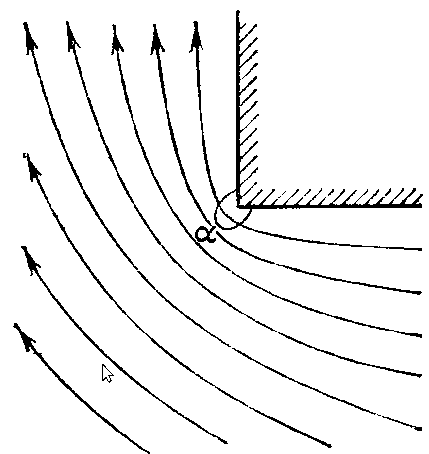
\includegraphics[width=6cm]{fig3}
  \caption{\label{fig:f3}}
\end{wrapfigure}

Член $Dxy$ может быть всегда исключен соответствующим поворотом осей $x$ и $y$.
В результате получаем:
\begin{equation}
   \label{eq:10t2}
   \varphi = Ax^2+By^2-(A+B)z^2.
\end{equation}
Если течение обладает аксиальной симметрией вокруг оси $z$ (симметричное
 обтекание тела вращения), то должно быть $A = B$, так что
\begin{equation}
   \label{eq:10t3}
   \varphi = A(x^2 + y^2 -2z^2).
\end{equation}
Компоненты скорости равны
\[
   v_x = 2Ax,
   v_y = 2Ay,
   v_z = -4Az,
\]
Линии тока определяются уравнениями (\ref{eq:5.2}), откуда $x^2z=c_1,\;y^2z=c_2$, т.е.
линии тока являются кубическими гиперболами.

Если течение является однородным вдоль оси $y$ (например, при обтекании в
направлении оси $z$ цилиндра с осью вдоль оси $y$), то в (\ref{eq:10t2}) должно быть $B=0$,
так что
\[
   \varphi = A(x^2 - z^2).
\]
Линиями тока являются гиперболы $xz = \const$.

\paragraph*{6}
Определить движение жидкости при потенциальном обтекании угла, образованного
двумя пересекающимися плоскостями  (вблизи вершины угла).

\texttt{Решение.} Выбираем полярные координаты $r,\theta$ в плоскости
поперечного сечеиия, перпендикулярной к линии пересечения плоскостей, с началом
в вершине угла. Угол $\theta$ отсчитывается от одной из прямых, образующих
сечение угла. Пусть $\alpha$ есть величина обтекаемого угла; при $\alpha<\pi$
течение происходит внутри угла, при $\alpha>\pi$ - вне его. Граничное условие
исчезновения нормальной составляющей скорости гласит $d\varphi/d\theta = 0$ при
$\theta = 0$ и $\alpha$. Удовлетворяющее этому условию решение уравнения Лапласа
пишем в виде \footnote{Выбираем решение с наиболее низкой (малые $r$!) положительной степенью $r$.}
\[
   \varphi = Ar^n\cos n\theta,\; n = \pi/\alpha,
\]
так что
\[
   v_r = nAr^{n-1}\cos n\theta,\; v_{\theta}=-nA^{n-1}\sin n\theta.
\]
При $n<1$ (обтекание выпуклого угла; рис. 3) $v$ обращается в начале координат
в бесконечность как $r^{-(1-n)}$. При $n>1$ (течение внутри вогнутого
угла - рис, 4) $v$; обращается при $r=0$ в нуль.

\begin{wrapfigure}{r}{6cm}
  \centering
  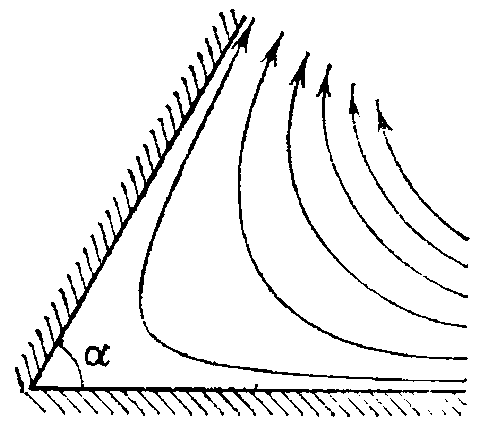
\includegraphics[width=6cm]{fig4}
  \caption{\label{fig:f4}}
\end{wrapfigure}

Функция тока, определяющая форму линий тока, есть
\[
   \psi = Ar^n \sin n\theta.
\]
Полученные для $\varphi$ п $\psi$ выражения являются вещественной и мнимой
частями комплексного по-тенииала $w = Az^n$ \footnote{Задачи 5 и 6, если рассматривать
граничные плоскости в них как бесконечные, вырождены в том смысле, что значения постоянных
коэффициентов $A,B$ в нх решениях остаются неопределенными. В реальных случаях обтекания
конечных тел эти значения определяются условиями задачи в целом.}.

\paragraph*{7}
Из несжимаемой жидкости, заполняющей все пространство, внезапно удаляется
сферический объем радиуса $a$. Определить время, в течение которого
образоваишаяся полость заполнится жидкостью  (\textit{Besant}, 1859;
\textit{Rayleigh}, 1917).

\texttt{Решение.} Движение жидкости после образования полости будет
центрально-симметрическим со скоростями, иаправлеииыми  в каждой точке по
 радиусу к центру.  Для радиальной скорости
\[
   v_r \equiv v<0
\]
имеем уравнение Эйлера (в сферических координатах)
\begin{equation}
   \label{eq:10t4}
   \pd{v}{t} + v \pd{v}{r} = - \frac1{\rho} \pd{p}{r}.
\end{equation}
Уравнение непрерывности дает:
\begin{equation}
   \label{eq:10t5}
   r^2v = F(t),
\end{equation}
где  $F(t)$ - произвольная функция времени; это равенство выражает собой тот
факт, что в силу несжимаемости жидкости объем, протекающий через сферу любого
радиуса, не зависит от последнего.

Подставляя $v$; из (\ref{eq:10t4}) в (\ref{eq:10t5}), имеем:
\[
   \frac{F'(t)}{r^2} + v \pd{v}{r} = - \frac1{\rho} \pd{p}{r},
\]
Интегрируя это уравнение по $r$ в пределах от $\infty$ до радиуса
\[
   R = R(t) \leq a
\]
заполняющейся полости, получим:
\begin{equation}
   \label{eq:10t6}
   - \frac{F'(t)}{R(t)} + \frac{V^2}{2} = \frac{p_0}{\rho},
\end{equation}
где $V = dR(t)/dt$ - скорость изменения радиуса полости, а $p_0$ - давление на
бесконечности; скорость жидкости на бесконечности, а также давление на
поверхности полости равны нулю. Написав соотношение (\ref{eq:10t5}) для точек на поверхности
полости, находим:
\[
   F(t) = R^2(t)V(t).
\]
и, подставив это выражение для $F(t)$ в (\ref{eq:10t6}), получим следующее уравнение
\begin{equation}
   \label{eq:10t7}
   - \frac{2V^2}{2} - \frac{1}{2} R \D{V^2}{R} = \frac{p_0}{\rho}.
\end{equation}
в этом уравнении переменные разделяются и, интегрируя его при начальном условии
$V=0$ при $R=a$ (в начальный момент жидкость покоилась), найдем:
\[
   V = \D{R}{t} = - \sqrt{\frac{2p_0}{3\rho}\left(\frac{a^3}{R^3}-1\right)}.
\]
Отсюда имеем для искомого полного времени заполнения полости:
\[
   \tau = \sqrt{\frac{3\rho}{2p_0}}\int_0^a{\frac{dR}{\sqrt{(a/R)^3}-1}}.
\]
Этот интеграл приводится к виду $B$-интеграла Эйлера, и вычисление дает
окончательно:
\[
   \tau = \sqrt{\frac{3a^2 \rho \pi}{2p_0}} \frac{\Gamma(5/6)}{\Gamma(1/3)} =
   0,915a \sqrt{\frac{\rho}{p_0}}.
\]

\paragraph*{8}
Погруженная в несжимаемую жидкость сфера расширяется по заданному закону
$R=R(t)$. Определить давление жидкости на поверхности сферы.

\texttt{Решение.} Обозначим искомое давление посредством $P(t)$. Вычисления в
точности аналогичны произведенным в предыдущей задаче с той лишь разницей, что
при $r=R$ давление равно не нулю, а $P(t)$. В результате получим вместо
(3) уравнение
\[
   - \frac{F'(t)}{R(t)} + \frac{V^2}{2} = \frac{p_0}{\rho} - \frac{P(t)}{\rho}
\]
и соответственно вместо (4) уравнение
\[
   \frac{p_0 - P(t)}{\rho} = - \frac{3V^2}{2} - RV \D{V}{R}.
\]
Имея в виду, что $V=dR/dt$, можно привести выражение для $P(t)$ к виду
\[
   P(t) = p_0 + \frac{\rho}{2}\left\lbrack \frac{d^2(R^2)}{dt^2} +
   \left( \D{R}{t} \right)^2 \right\rbrack.
\]

\paragraph*{9}
Определить  форму  струн,  вытекающей   из   бесконечно  длинной   щели
прорезанной в плоской стенке.
\texttt{Решение.} Пусть в плоскости $x,y$ стенка совпадает с осью $x$,
отверстие есть отрезок $-a/2 \leq x \leq a/2$ этой оси, а жидкость занимает
полуплоскость $y>0$. Вдали от стенки (при $y \to \infty$) скорость жидкости
равна нулю, а давление пусть будет $p_0$.

\begin{figure}[hb]
  \centering
  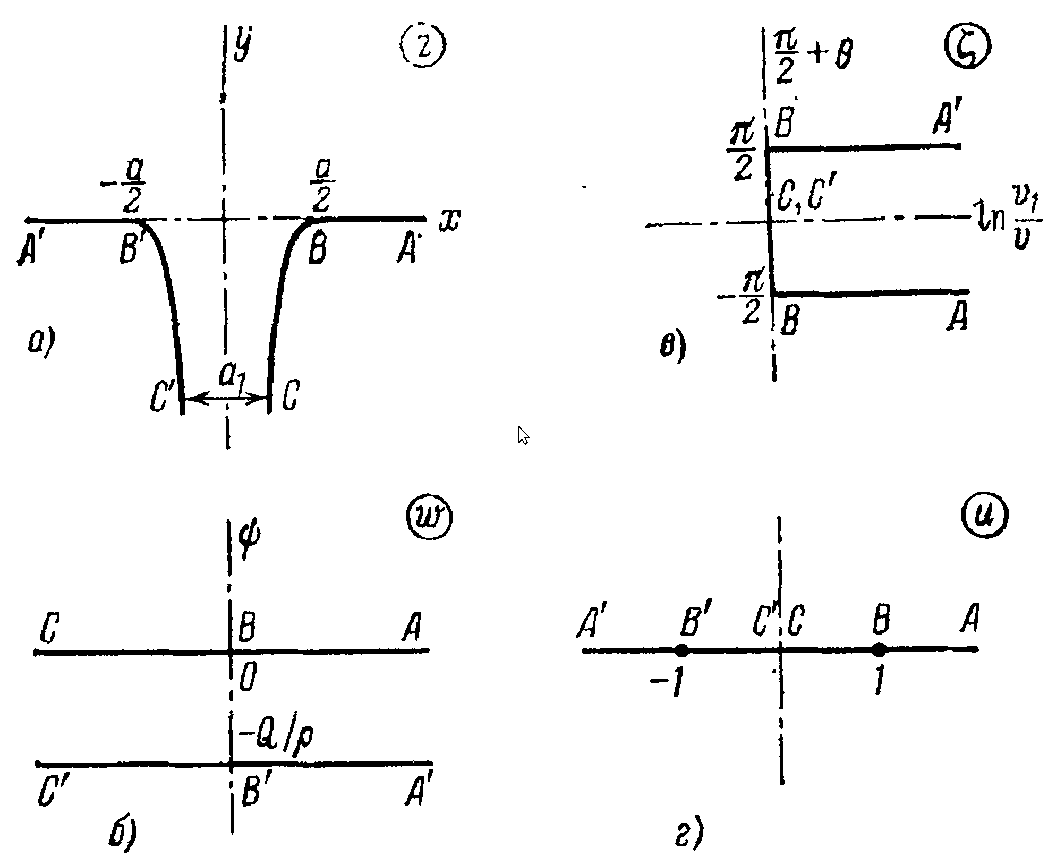
\includegraphics[width=9cm]{fig5}
  \caption{\label{fig:f5}}
\end{figure}

На свободной поверхности струя ($BC$ и $B'C'$ на рис. 5,а) давление $p=0$, а
скорость согласно уравнению Бернулли имеет постоянную величину $v_1 =
\sqrt{2p_0/\rho}$. Линии стенки, продолжающиеся в свободную границу струи,
представляют собой линии тока. Пусть на лниии $ABC$ $\psi = 0$; тогда на линии
$A'B'C'$ $\psi = -Q/\rho$. Где $Q = \rho a_1 v_1$ - расход жидкости в струе
($a_1$, $v_1$ - ширина струн и скорость жидкости в ней на бесконечности).
Потенциал $\varphi$ меняется как на линии $ABC$, так и на линии $A'B'C'$ от
$-\infty$ до $+\infty$; пусть в точках $B$ и $B' \varphi = 0$, Тогда в плоскости
комплексного переменного $w$ области течения будет соответствовать бесконечная
полоса ширины $Q/\rho$ (обозначения точек на рис, 5,б - г соответствуют
обозначениям на рис, 5,а в плоскости $x,y$). Введем новую комплексную переменную
- логарифм комплексной скорости:
\begin{equation}
   \label{eq:10t9.1}
   \zeta = - \ln \left\lbrack \frac1{v_1 e^{i\pi/2}} \D{w}{z} \right\rbrack =
   \ln \frac{v_1}{v} + i \left( \frac{\pi}{2} + \theta \right)
\end{equation}
($v_1 e^{i\pi/2}$ - комплексная скорость на бесконечности струи). На $A'B'$
имеем $\theta = 0$; на $AB \theta = - \pi$ на $BC$ и $B'C'$ $v=v_1$, причем на
бесконечности струн $\theta = - \pi/2$. Поэтому в плоскости переменного $\zeta$
области течения соответствует полуполоса ширины $\pi$, расположенная в правой
полуплоскости (рис, 5, в). Если мы теперь найдем конформное преобразование,
переводящее полосу плоскости $w$ в полуполосу плоскости $\zeta$ (с указанным на
рис. 5 соответствием точек), то тем самым мы определим $w$ как функцию от
$dw/dz$; функция $w$ может быть найдена затем одной квадратурой.

Для того чтобы найти искомое преобразование, введем еще одну вспомогательную
комплексную переменную $u$, такую, чтобы в плоскости $u$ области течения
соответствовала верхняя полуплоскость, причем точкам $B$ и $B'$ соответствуют
точки $u=\pm 1$, точкам $C,C'\; u = 0$, а бесконечно удаленным точкам $A$ и $A'$
$u = \pm \infty$ (рис, 5,г). Зависимость $w$ от этой вспомогательной переменной
определяется конформным преобразованием, переводящим верхнюю полуплоскость $u$ в
полосу плоскости $w$. При условленном соответствии точек это есть
\begin{equation}
   \label{eq:10t9.2}
   w = - \frac{Q}{\rho\pi}\ln u
\end{equation}
Чтобы найти зависимость $\zeta$ от $u$, надо найти конформное отображение
полуполосы плоскости $\zeta$, в верхнюю полуплоскость $u$. Рассматривая эту
полуполосу как треугольник, одна из вершин которого удалена в бесконечность,
можно найти искомое отображение с помощью известной формулы Шварца-Кристоффеля;
ответ гласит
\begin{equation}
   \label{eq:10t9.3}
   \zeta = - i \arcsin u.
\end{equation}
Формулы (\ref{eq:10t9.2}), (\ref{eq:10t9.3}) решают задачу, определяя в параметрическом виде зависимость
$dw/dz$ от $w$.

Определим форму струи. На $BC$ имеем
$w = \varphi,\; \zeta = i \left( \frac{\pi}{2}+\theta \right) $, а $u$
меняется между 0 и 1. Из (\ref{eq:10t9.2}) и (\ref{eq:10t9.3}) получим:
\begin{equation}
   \label{eq:10t9.4}
   \varphi = - \frac{Q}{\rho \pi}\ln (-\cos \theta),
\end{equation}
а из (1) $d\varphi/dz = v_1 e^{-i\theta}$, или
\[
   dz \equiv dx + i\; dy = \frac1{v_1} e^{i\theta}d\varphi =
   \frac{a_1}{\pi} e^{i\theta} \tan \theta\; d\theta,
\]
откуда интегрированием (с условиями $y=0, x=a/2$ при $\theta = - \pi$) найдем
в параметрическом виде форму струи, В частности, для сжатия струи получается
$a_1/a = \pi/(2+\pi) = 0,61$.


